\documentclass[preprint,12pt]{elsarticle}

    \usepackage[sc]{mathpazo} % Use the Palatino font
    \usepackage[T1]{fontenc} % Use 8-bit encoding that has 256 glyphs
    \usepackage{microtype} % Slightly tweak font spacing for aesthetics
    \usepackage[english]{babel} % Language hyphenation and typographical rules
    \usepackage{booktabs} % Horizontal rules in tables
    \usepackage{enumitem} % Customized lists
    \usepackage[table,xcdraw]{xcolor}
    \usepackage[utf8]{inputenc} % Required for inputting international characters
    \usepackage{parskip}
    \usepackage{graphicx}
    \usepackage{hyperref}
    \usepackage{pdfpages}
    \usepackage{amsmath}
    \usepackage{esvect}
    \usepackage{listings}
    \usepackage{color}
    \usepackage{spverbatim}
    \usepackage{subcaption}
    \usepackage{multirow}
    \usepackage[title]{appendix}
    \hypersetup{
        colorlinks=true,
        linkcolor=blue,
        filecolor=magenta,      
        urlcolor=cyan,
    }
    \definecolor{dkgreen}{rgb}{0,0.6,0}
    \definecolor{gray}{rgb}{0.5,0.5,0.5}
    \definecolor{mauve}{rgb}{0.58,0,0.82}
    \definecolor{lightgray}{rgb}{0.83, 0.83, 0.83}
    \definecolor{timberwolf}{rgb}{0.86, 0.84, 0.82}
    \definecolor{whitesmoke}{rgb}{0.96, 0.96, 0.96}
    
    \lstset{frame=tb,
    language=python,
    aboveskip=3mm,
    belowskip=3mm,
    showstringspaces=false,
    columns=flexible,
    basicstyle={\small\ttfamily},
    numbers=none,
    numberstyle=\tiny\color{gray},
    keywordstyle=\color{blue},
    commentstyle=\color{dkgreen},
    stringstyle=\color{mauve},
    breaklines=true,
    breakatwhitespace=true,
    tabsize=3,
    backgroundcolor = \color{whitesmoke}
    }

    \begin{document}
    \title{\LARGE \bf
        STAT 391 Homework 6
        }
        
        \author{ \parbox{3 in}{\centering Chongyi Xu \\
                 University of Washington\\
                 STAT 391 Spring 2018\\
                 {\tt\small chongyix@uw.edu}}
        }
    \maketitle

    \section{Problem 1 - Statistical decision making}
    \begin{enumerate}[label=\alph*]
        \item Make a neatly labeled table of the outcome space for
        this problem.
        \begin{table}[h!]
			\centering
			\begin{tabular}{|l|l|}
				\hline
				1st Day(Room B)                        & 2nd Day(Room A)       \\ \hline
				$F,G|B$                          & --            \\ \hline
				$!F,G|B$						& $!F|B$		\\ \hline
				\multirow{3}{*}{$!F,G|A$} & $F,G|A$         \\ \cline{2-2} 
											   & $F,!G|A$ \\ \cline{2-2} 
											   & $!F|A$   \\ \hline
			\end{tabular}
			\caption{Outcome Space}
			\label{table1}
		\end{table}
		Table\ref{table1} is the outcome space.

        \item What is the probability that Rob finds the graphics card
        on the second day?
        \begin{align*}
			P(F\text{ on the second day}) &= P(\bar{F}|B) * P(F|A) * P(A)\\
			&= 1\cdot \frac{1}{2} \cdot \frac{1}{3} = \frac{1}{6}
        \end{align*}

		\item What is the probability that he finds the graphics card?
		\begin{align*}
			P(F) &= P(F|A) + P(F|B) \\
			&= \frac{1}{2} + \frac{2}{5}\\
			&= \frac{9}{10}
		\end{align*}
		
		\item What is the probability that he finds the card and the card
		is still good?
		\begin{align*}
			P(F,G) &= P(F|B) \cdot P(G|B) + P(F|A) \cdot P(G|A)\\
			&= \frac{2}{5} + \frac{1}{2}\cdot \frac{4}{5}\\
			&= \frac{4}{5}
		\end{align*}

		\item What is the expected value of Rob's search policy?
		\begin{table}[h!]
			\centering
			\begin{tabular}{|l|l|}
				\hline
				1st Day(Room B)                        & 2nd Day(Room A)       \\ \hline
				$F,G|B = \frac{2}{5}\cdot \frac{2}{3} = \frac{4}{15}$                          & --            \\ \hline
				$!F,G|B = \frac{3}{5}\cdot \frac{2}{3} = \frac{6}{15}$						& $!F|B=1$		\\ \hline
				\multirow{3}{*}{$!F,G|A = 1$} & $F,G|A = \frac{1}{2}\cdot \frac{1}{3}\cdot \frac{4}{5} = \frac{2}{15}$         \\ \cline{2-2} 
											   & $F,!G|A = \frac{1}{2}\cdot \frac{1}{3}\cdot \frac{1}{5} = \frac{1}{30}$ \\ \cline{2-2} 
											   & $!F|A = \frac{1}{2}\cdot \frac{1}{3} = \frac{1}{6}$   \\ \hline
			\end{tabular}
			\caption{Outcome Space with probability}
			\label{table2}
		\end{table}
		\\ Considering the outcome space with probability Table\ref{table2}. So the expectation value is
		\begin{align*}
			E(\text{policy}) &= \frac{4}{15}\times (+60-10) + \frac{6}{15}\cdot 1\times (-10-10\times 2 -5)\\
			&\qquad + 1\cdot \frac{2}{15}\times (+60-10\times 2 - 5) + 1\cdot \frac{1}{30}\times (0-10\times 2 - 5)\\
			&\qquad + 1\cdot \frac{1}{6}\times (-10-10\times 2 - 5)\\
			&=-\frac{8}{3}\approx -2.67
		\end{align*}

		\item Help Rob compare the following policies:
		\\ Plan 1: Search B on 1st day, search A on 2nd day if necessary.
		\\ Plan 2: Search A on 1st ady, search B on 2nd day if necessary.
		\\ Plan 3: Search B on 1st day, don't search 2nd day.
		\\ Plan 4: Search A on 1st day, don't search 2nd day.
		\\ Plan 5: Don't search at all!
		\\ Rob would still have to choose his own decision criteria. Justify your answer by showing your reasoning or your calculations in all cases.

		From part(e), we have found the $E(\text{Plan 1}) = -\frac{8}{3}$.
		\begin{align*}
			E(\text{Plan 2}) &= \frac{1}{2\times 3}\times (+60-10) + \frac{1}{2\times 3}\cdot 1\times (-10-10\times 2 -5)\\
			&\qquad + 1\cdot \frac{2\times 2\times 3}{3\times 5\times 5}\times (+60-10\times 2 - 5)\\
			&\qquad + 1\cdot \frac{2\times 2\times 2}{3\times 5\times 5}\times (0-10\times 2 - 5)\\
			&\qquad + 1\cdot \frac{2\times 3}{3\times 5}\times (-10-10\times 2 - 5)\\
			&\approx -8.57\\
			E(\text{Plan 3}) &= \frac{2}{5}\cdot \frac{2}{3}\times (+60-10) + \frac{3}{5}\cdot \frac{2}{3}\times (-10-10) + \frac{1}{3}\times (-10-10)\\
			&\approx -1.33\\
			E(\text{Plan 4}) &= \frac{1}{2} \cdot \frac{1}{3}\times (+60-10) + \frac{1}{2} \cdot \frac{1}{3}\times (-10-10) + \frac{2}{3}\times (-10-10)\\
			&\approx -8.33\\
			E(\text{Plan 5}) &= -10
		\end{align*}
		Therefore, the best optimized policy is Plan 3 by maximizing the expected gain.

		
	\end{enumerate}
	
	\section{Problem 3- Bayesian Inference}
	\begin{enumerate}[label=\alph*]
		\item Compute the probability that a customer buys all three
		books under $\bar{P}_{ABC}$.
		\begin{equation*}
			\bar{P}_{ABC}(1,1,1) = 0.6\cdot 0.3\cdot 0.4 = 0.072
 		\end{equation*}
		 
		\item Compute the probability that a customer buys all three
		books under $\tilde{P}$
		\begin{equation*}
			\tilde{P}_{ABC}(1,1,1) = 0.1\cdot 0.4 = 0.04
		\end{equation*}
		 
		\item Using $\bar{P}$ and $\tilde{P}$ from above, determine if 
		the likelihood that Robin Hood is a man is higher than the 
		likelihood that the (s)he's a woman.
		\begin{align*}
			\bar{P}_{ABC}(1,1,0) &= 0.6\cdot 0.3\cdot (1-0.4) = 0.108\\
			\tilde{P}_{ABC}(1,1,0) &= 0.1\cdot (1-0.4) = 0.06
		\end{align*}
		Therefore, the likelihood tells Robin Hood is more likely to be 
		a woman.

		\item Determine the posterior probability that Robin Hood is a man.
		\begin{align*}
			P(man|A=1,B=1,C=0) &= \frac{P((1,1,0)|man)P(man)}{P(1,1,0)}\\
			&= \frac{0.06\cdot \frac{2}{3}}{0.06+0.108}\\
			&= \frac{0.04}{0.168}\\
			&\approx 0.238
		\end{align*}

		\item Determine the posterior probability that RObin Hood is a man if 
		Al doesn't recall whether Robin ordered Book C or not.
		\begin{align*}
			P(man|(1,1)) &= P(man|(1,1,1)) + P(man|(1,1,0))\\
			&= \frac{P((1,1,1)|man)P(man)}{P(1,1,1)} + 0.238\\
			&= \frac{0.04\cdot \frac{2}{3}}{0.112} + 0.238\\
			&= 0.238 + 0.238 = 0.476
		\end{align*}

		\item Compute the value of Likelihood Ratio(LR) for the data $A=1,B=1,C=0$
		\begin{equation*}
			LR(A=1,B=1,C=0) = \frac{\bar{P}_{ABC}(1,1,0)}{\tilde{P}_{ABC}(1,1,0)} = \frac{0.108}{0.06} = 1.8
		\end{equation*}

		Compute the value of the LR if the data consists of 3 customers 
		$A_1=1,B_1=0,C_1=0,A_2=0,B_2=1,C_2=0,A_3=1,B_3=0,C_3=1$.
		\begin{align*}
			LR(D) &= \frac{\bar{P}_{ABC}(1,0,0)\cdot \bar{P}_{ABC}(0,1,0)\cdot \bar{P}_{ABC}(1,0,1)}{\tilde{P}_{ABC}(1,0,0)\cdot \tilde{P}_{ABC}(0,1,0)\cdot \tilde{P}_{ABC}(1,0,1)}\\
			&= \frac{0.6*(1-0.3)*(1-0.4)*(1-0.6)*0.3*(1-0.4)*0.6*(1-0.3)*0.4}{0.5*(1-0.4)*0.2*0.6*0.5*0.4}\\
			&= 0.423
		\end{align*}

		\item Give an example of a data set where $LR>1$.
		\begin{equation*}
			D:A_1=1,B_1=1,C_1=0,A_2=1,B_2=1,C_2=1
		\end{equation*}
		
	\end{enumerate}

	\section{Problem 5 - Dirichlet/Beta Distribution}
	\begin{enumerate}[label=\alph*]
		\item Change the variables $\theta_j$ to $\xi_j=ln \theta_j$ and express
		$L$ as a function of $\xi$.
		\begin{equation*}
			L = P(\theta_1,\theta_2) = \theta_1^{n_1}\theta_2^{n_2} = n_1\xi_1 n_2\xi_2
		\end{equation*}

		\item Let $m=2,S=\{1,2\}, $and $D=\{1,1,2,1,1\}$. For the following 3 dirichlet priors, give numerical values of the fictitious sample size $\alpha$, and the posterior parameters $\alpha_{1,2}^{'}$

		\begin{itemize}
			\item $Diri(\theta_1,\theta_2;0.9,0.1)$
			\\ For this case, $\alpha=0.9+0.1=1$, $\alpha_1^{'}=0.9+4=4.9$,
			$\alpha_2^{'}=0.1+1=1.1$

			\item $Diri(\theta_1,\theta_2;2,3)$
			\\ For this case, $\alpha=2+3=5$, $\alpha_1^{'}=2+4=6$,
			$\alpha_2^{'}=3+1=4$

			\item $Diri(\theta_1,\theta_2;20,20$
			\\ For this case, $\alpha=20+20=40$, $\alpha_1^{'}=20+4=24$,
			$\alpha_2^{'}=20+1=21$
		\end{itemize}

		\item Let $\theta=\theta_2$. For each of the 3 cases above, make a plot 
		showing the prior, posterior as functions of $\theta$, as well as
		the location of ML estimate $\theta_2^{ML}$ on the $\theta$ axis.
		\begin{figure}[h!]
            \center
            \begin{subfigure}{0.48\textwidth}
                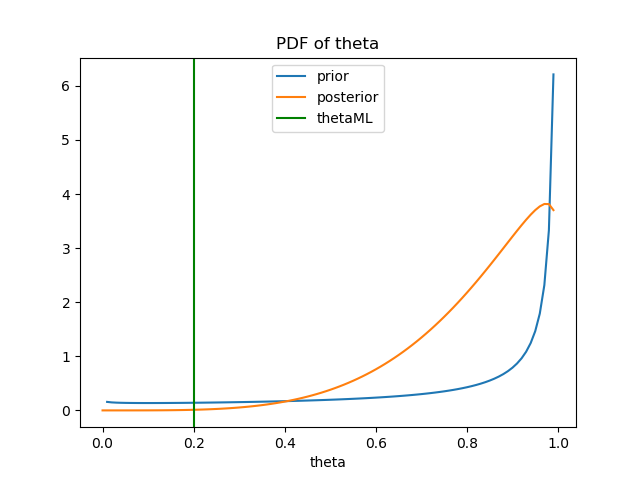
\includegraphics[width = \textwidth]{1.png}
                \caption{PDF of $theta$ for case $Diri(\theta_1,\theta_2;0.9,0.1)$}
                \label{fig:11}
            \end{subfigure}
            \begin{subfigure}{0.48\textwidth}
                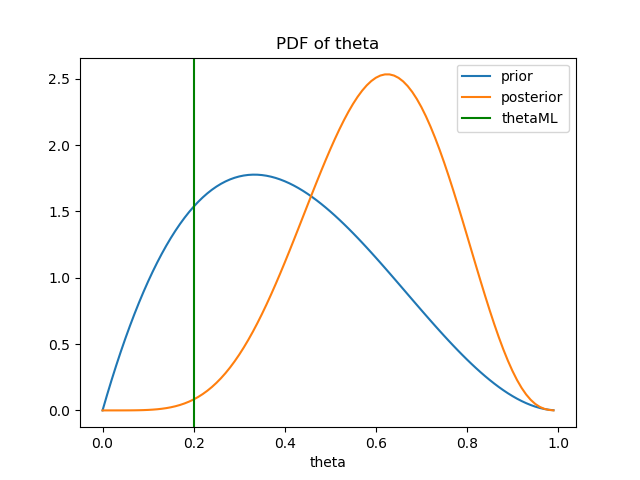
\includegraphics[width = \textwidth]{2.png}
                \caption{PDF of $theta$ for case $Diri(\theta_1,\theta_2;2,3)$}
                \label{fig:12}
			\end{subfigure}
			\begin{subfigure}{0.48\textwidth}
				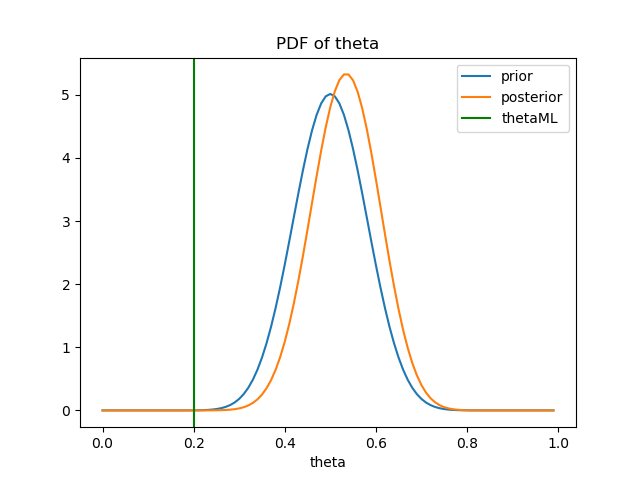
\includegraphics[width=\textwidth]{3.png}
				\caption{PDF of $theta$ for case $Diri(\theta_1,\theta_2;20,20)$}
				\label{fig:13}
			\end{subfigure}
			\caption{Estimation of logistic density}
            \label{fig:1}
		\end{figure}
		
		\item Assume now the prior is uniform, that is $Diri(\theta_1,\theta_2;1,1)$.
		Show that the posterior of $(\theta_1,\theta_2)$ is a Beta distribution and 
		calculate its parameters for the data in \textbf{b}.
		\\ Consider we have a data set with $n_1$ observations of outcome 1 and $n_2$
		observations of outcome 2. Then the posterior of $(\theta_1,\theta_2)$ is
		\begin{align*}
			Diri(\theta_1,\theta_2;1+n1,1+n2) &= \frac{\Gamma(1+n1)}{\Gamma(1+n1)\Gamma(1+n2)}
			\theta_1^{n1}\theta_2^{n2}\\
			&= Beta(\theta_1,\theta_2;1+n1,1+n2)
		\end{align*}
		So the posterior parameters for data in \textbf{b} is $\alpha_1^{'}=1+4=5$,$\alpha_2^{'}=1+1=2$.

		\item Same as \textbf{c}, plot prior, posterior and location of ML estimate for 
		$\theta_2^{ML}$ for the uniform prior.
		\begin{figure}[h!]
            \center
			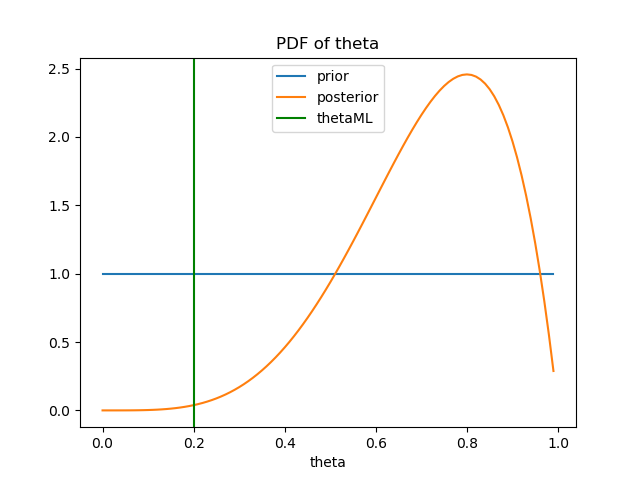
\includegraphics[width=0.8\textwidth]{4.png}
			\caption{PDF of $\theta$ for $Diri(\theta_1,\theta_2;5,2)$}
			\label{fig:2}
		\end{figure}
		\\Figure\ref{fig:2} shows the plot.

	\end{enumerate}

\end{document}